	\section*{Exercice 2 (5 points)}
	
	\subsection*{1. Quel pourcentage de la production totale le sous-traitant B assure-t-il ?}
	
	Le sous-traitant B assure $100 - 40 = \numprint{60}$\% de la production totale.
	
	\subsection*{2. Quelle est la probabilité qu’un téléphone provienne du sous-traitant B sachant qu’il est défectueux ? On arrondira le résultat à $10^{-3}$ près.}
	
	On peut dresser un arbre pondéré de probabilités en posant :
	\begin{itemize}
		\item $A$ l’évènement : « le téléphone provient du sous-traitant A » ;
		\item $T$ l’évènement : « le téléphone est défectueux ».
	\end{itemize}
	
	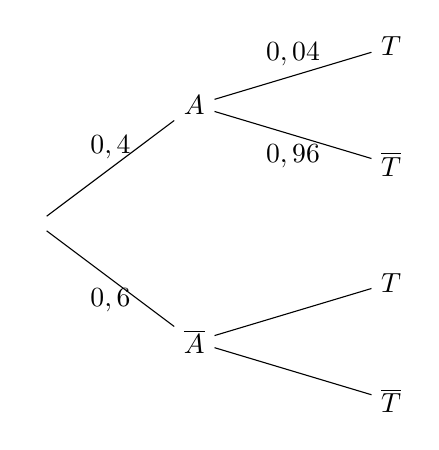
\begin{tikzpicture}
		[level 1/.style={level distance=2cm,
			sibling distance=3cm},
		level 2/.style={level distance=2.5cm,
			sibling distance=1.5cm}]
		\node {} [grow'=right]
		child {node {$A$}
			child {node {$T$}
				edge from parent node[above] {$0,04$}
			}
			child {node {$\overline T$}
				edge from parent node[below] {$0,96$}
			}
			edge from parent node[above] {$0,4$}
		}
		child {node {$\overline A$}
			child {node {$T$}
				edge from parent node[above] {}
			}
			child {node {$\overline T$}
				edge from parent node[below] {}
			}
			edge from parent node[below] {$0,6$}
		}
		;
	\end{tikzpicture}
	
	D’après la loi des probabilités totales :
	\[
	P(T) = P(A \cap T) + P(\overline{A} \cap T)
	\]
	
	Avec $P(T) = 0,034$ et $P(A \cap T) = 0,4 \times 0,04 = 0,016$, l’égalité ci-dessus devient :
	\[
	0,034 = 0,016 + P(\overline{A} \cap T) \quad \text{d’où} \quad P(\overline{A} \cap T) = 0,034 - 0,016 = 0,018
	\]
	
	Il faut trouver $P_T(\overline{A}) = \dfrac{P(T \cap \overline{A})}{P(T)} = \dfrac{0,018}{0,034} = \dfrac{18}{34} = \dfrac{9}{17} \approx 0,529$, soit $\numprint{0.529}$ au millième près.
	
